\documentclass[a4paper,12pt,oneside]{book}
\usepackage[utf8]{inputenc}
\usepackage{times}
\usepackage{amssymb} 
\usepackage{amsmath}
\usepackage{listings}
\usepackage{color}
\usepackage{cite}
\usepackage{amsmath,amssymb,amsfonts}
\usepackage{algorithmic}
\usepackage{graphicx}
\usepackage{textcomp}
\usepackage{xcolor}
\usepackage{amsmath}
\DeclareMathOperator*{\maxi}{max}
\def\BibTeX{{\rm B\kern-.05em{\sc i\kern-.025em b}\kern-.08em
    T\kern-.1667em\lower.7ex\hbox{E}\kern-.125emX}}
\definecolor{codegreen}{rgb}{0,0.6,0}
\definecolor{codegray}{rgb}{0.5,0.5,0.5}
\definecolor{codepurple}{rgb}{0.58,0,0.82}
\definecolor{backcolour}{rgb}{0.95,0.95,0.92}
\lstdefinestyle{mystyle}{
    backgroundcolor=\color{backcolour},   
    commentstyle=\color{codegreen},
    keywordstyle=\color{magenta},
    numberstyle=\tiny\color{codegray},
    stringstyle=\color{codepurple},
    basicstyle=\footnotesize,
    breakatwhitespace=false,         
    breaklines=true,                 
    captionpos=b,                    
    keepspaces=true,                 
    numbers=left,                    
    numbersep=9pt,                  
    showspaces=false,                
    showstringspaces=false,
    showtabs=false,                  
    tabsize=2
}

\lstset{style=mystyle}
\usepackage{graphicx}
\usepackage{float}
\usepackage[export]{adjustbox}
\graphicspath{ {images/} }
\usepackage{times}
\usepackage{geometry}
\usepackage{setspace}
\usepackage{tocloft}
\usepackage{tabu}
\usepackage{fancyhdr}
\geometry{
    left=35mm,   % Left margin
    right=25mm,  % Right margin
    top=25mm,    % Top margin
    bottom=25mm  % Bottom margin
}
\usepackage{titlesec}
\usepackage[toc,page]{appendix}
\titleformat{\chapter}[display]
  {\normalfont\huge\centering}
  {\chaptertitlename\ \thechapter}{16pt}{\Huge}

\fancypagestyle{frontmatter}{
    \fancyhf{} % Clear header and footer
    \renewcommand{\headrulewidth}{0pt} % Remove header rule
    \renewcommand{\footrulewidth}{0pt} % Remove footer rule
    \cfoot{\thepage} % Centered page number (Roman numerals)
}

% Define page style for main matter
\fancypagestyle{mainmatter}{
    \fancyhf{} % Clear header and footer
    \renewcommand{\headrulewidth}{0pt} % Remove header rule
    \renewcommand{\footrulewidth}{0pt} % Remove footer rule
    \cfoot{\thepage} % Centered page number (Arabic numerals)
}

% Front matter
\pagenumbering{roman} % Use Roman numerals for page numbering
\pagestyle{frontmatter} % Use 'frontmatter' page style



\renewcommand{\cftchapleader}{\cftdotfill{\cftdotsep}} % for chapters
\renewcommand\contentsname{\centerline{INDEX}}
\pagestyle{fancy}
\cfoot{\thepage}
\rhead{}
\lhead{}
\renewcommand{\headrulewidth}{0pt}
\renewcommand{\footrulewidth}{0pt}
% Here you can insert your BTP Title here
\newcommand{\btptitle}{BUILDING A VIABLE AI-GENERATED IMAGE DETECTION MODEL USING METAHEURISTIC ALGORITHMS}







\begin{document}
% Change the title below to your own title E.g. \title{MYPROJECTNAME}

\title{\btptitle}
\mainmatter
% \tableofcontents
% \section{Intro}
% yo yo
\addtocontents{toc}{{Title}\hfill{Page No.}\par}
\begin{titlepage}
\begin{center}
% Insert your project title where it says {PROJECT TITLE}
\fontsize{15pt}{1cm}\selectfont {\btptitle}

\vspace*{1.4cm}
\fontsize{15pt}{21pt}\selectfont A REPORT 
\\ SUBMITTED IN PARTIAL FULFILLMENT OF THE \\ REQUIREMENTS \\ FOR THE AWARD OF THE DEGREE \\ OF \\ BACHELOR OF TECHNOLOGY \\
IN \\ DEPARTMENT OF INFORMATION TECHNOLOGY 


\vspace*{0.6cm}
Submitted By\\
% Insert your name here under Name 1 and Name 2 as well as your respective Roll Numbers.
% To insert another name add this before the } --> \\NAME 3 (ROLL NUMBER)
\fontsize{15pt}{21pt}\selectfont {STUBH LAL (Roll No.: 2020UIT3116)\\MANIK (Roll No.: 2020UIT3124)\\ SIPPU UTKARSH (Roll No.: 2020UIT3137)} \linebreak
\\Under the supervision of\\
% Insert your name here under Name 1 and Name 2 as well as your respective Roll Numbers.
% To insert another name add this before the } --> \\NAME 3 (ROLL NUMBER)
\textbf{Dr. Priti Bansal}

\vspace*{0.2cm}
\includegraphics[width=2in]{images/nsut.png}

\vspace*{0.3cm}
% Insert Department Name where it says DEPARTMENT NAME
\fontsize{15pt}{16pt}\selectfont {DIVISION OF INFORMATION TECHNOLOGY\\NETAJI SUBHAS UNIVERSITY OF TECHNOLOGY\\MAY 2024}

\end{center}
\end{titlepage}
\pagenumbering{roman} 
\pagestyle{mainmatter} % Use 'mainmatter' page style

\addcontentsline{toc}{chapter}{DECLARATION}
\thispagestyle{plain}
\begin{center}
\large \large {DECLARATION}

\end{center}
\begin{center}
   \includegraphics[width=2in]{images/nsut.png} 
\end{center}

\begin{center}
  \fontsize{12pt}{24pt}\selectfont{Department of Information technology\\Delhi-110078, India } 
 
\end{center}
\vspace{0.3cm}
% Enter the title of your project in the main.tex file where it says PROJECT NAME
\fontsize{12pt}{24pt}\selectfont We, Stubh Lal (2020UIT3116), Manik (2020UIT3124), Sippu Utkarsh (2020UIT3137),  students of B. Tech., Department of Information  Technology, hereby declare that the Project II - Thesis titled \textbf{“Building a viable AI-generated image detection model using metaheuristic algorithms” }which is submitted  by us to the Department of Information Technology, Netaji Subhas University of Technology,  in partial fulfillment of the requirement for the award of the degree of Bachelor of Technology, is  original and not copied from source without proper citation. This work has not previously formed  the basis for the award of any Degree. 

\vspace{2.0cm}


\begin{tabu} to \textwidth { X[l] X[c] }

Place: & (Name and Signature of Students) 
 
\end{tabu}

\fontsize{12pt}{24pt}\selectfont{Date: } 


\newpage

\addcontentsline{toc}{chapter}{CERTIFICATE}
\thispagestyle{plain}
\begin{center}
\large \large {CERTIFICATE}

\end{center}
\begin{center}
   \includegraphics[width=2in]{images/nsut.png} 
\end{center}

\begin{center}
  \fontsize{12pt}{24pt}\selectfont{Department of Information technology\\Delhi-110078, India } 
 
\end{center}
\vspace{0.3cm}
% Enter the title of your project in the main.tex file where it says PROJECT NAME
\fontsize{12pt}{24pt}\selectfont This is to certify that the work embodied in the Project II-Thesis titled \textbf{“Building a viable AI-generated image detection model using metaheuristic algorithms”} has  been completed by Stubh Lal (2020UIT3116), Manik (2020UIT3124), Sippu Utkarsh (2020UIT3137), students of B.Tech., Department of  Information Technology, under my guidance towards fulfilment of the requirements for the  award of the degree of Bachelor of Technology. This work has not been submitted for any other  diploma or degree of any University. 


\vspace{2.0cm}


\begin{tabu} to \textwidth { X[l] X[c] }

Place: & (Name and Signature of Supervisor) 
 
\end{tabu}

\fontsize{12pt}{24pt}\selectfont{Date: } 


\newpage
\addcontentsline{toc}{chapter}{ABSTRACT}
\thispagestyle{plain}
\begin{center}
\large \large {ABSTRACT}

\end{center}

\fontsize{12pt}{24pt}\selectfont {Synthetic image generation has advanced significantly in recent years because of several breakthroughs in Artificial Intelligence (AI) technologies such as deep learning with images being generated exhibiting diversity as well as high quality. As a result, it is absolutely necessary to develop a tool that can accurately distinguish between real images and synthetic AI-generated images. The study proposes a framework involving feature extraction from the images of a publicly available dataset CIFAKE by using Convolutional Neural Networks and after comparison of several pre-trained models, we choose the best pre-trained model, ResNet152V2 and after comparison of several metaheuristic optimization algorithms, we select Coral Reef Optimization for feature selection. Following the fine-tuning of the model, the accuracy obtained by this approach was  97.315\% which is better than the recent works on the same dataset.}

\newpage


\addcontentsline{toc}{chapter}{INDEX}
\tableofcontents
\newpage

\addcontentsline{toc}{chapter}{LIST OF TABLES}
\thispagestyle{plain}

\section*{}
\begin{center}
\large \large {LIST OF TABLES}
\end{center}


\begin{table}[H]
\begin{tabular}{|l|l|l|}
\hline
S.No & Table                         & Page Number \\ \hline
1.   & Data Augumentation Parameters & 25          \\ \hline
2.   & Initial Training Results      & 33         \\ \hline
3.   & Metaheuristic Comparison      & 36          \\ \hline
4.   & Final Results                 & 39          \\ \hline
\end{tabular}
\end{table}

\newpage

\addcontentsline{toc}{chapter}{LIST OF FIGURES}
\thispagestyle{plain}

\section*{}
\begin{center}
\large \large {LIST OF FIGURES}
\end{center}


\begin{table}[H]
\begin{tabular}{|l|l|l|}
\hline
S.No & Table                         & Page Number \\ \hline
1.   & A residual block     & 14          \\ \hline
2.   & MobileNet Convolution    & 16          \\ \hline
3.   & DenseNet      & 17          \\ \hline
4.   & Visualization of Particle Swarm Optimization                 & 19         \\ \hline
5.   & Genetic Algorithm Representation    & 20         \\ \hline
6.   & Crossover and Mutation         & 20          \\ \hline
7.   & An AI-generate image of a hand             & 21          \\ \hline
8.   & Examples of real images from CIFAR-10 Image Classification Dataset                 & 23         \\ \hline
9.   & Examples of AI - Generated images from CIFAKE Dataset                & 23         \\ \hline
10.   & Model Summary                 & 25          \\ \hline
11.   & Confusion Matrix of best model: ResNet152V2              & 34          \\ \hline
12.   & Training ResNet152V2 with top layers frozen                 & 34         \\ \hline
13.   & Fine-tuning ResNet152V2 with top layers unfrozen           & 35         \\ \hline
14.   & Graphic results of metaheuristic. comparison               & 35          \\ \hline
15.   & Training the final model with top layers frozen             & 37          \\ \hline
16.   & Fine-tuning the final model with top layers unfrozen                 & 37          \\ \hline
17.   & Receiver Operating Characteristic & 38          \\ \hline
18.   & Confusion Matrix for the Final Model   & 38          \\ \hline

\end{tabular}
\end{table}

\newpage

% Create chapters by first adding a new .tex file with your chapter name. E.g. <ChapterFileName>.tex
% Insert your chapters here in the format specified below
% \chapter{ChapterName}
% \input{ChapterFileName}
% This will ensure that your chapter will be added to the table of contents

\pagenumbering{arabic} % Switch to Arabic numerals for page numbering
\pagestyle{mainmatter} % Use 'mainmatter' page style

\chapter{Introduction}

\section{Background}

In recent years, advancements in Artificial Intelligence (AI) have propelled the rapid growth of synthetic image creation. These advancements, which have been made in AI-generated images by researchers, have improved the quality, diversity as well as realism of generated images over the years. AI-generated images find applications in several domains such as art generation, image editing, content creation and data augmentation. Techniques of style transfer, attention mechanisms and progressive growing have even strengthened the capabilities of image generation models, enabling the generation of photorealistic images. 

Generative Adversarial Networks revolutionized the field of image generation in 2014 \cite{goodfellow}, changing the way synthetic content is created. These networks consist of two neural networks : a generator and a discriminator which compete against one another through adversarial training. However, these networks faced several challenges and limitations of mode collapse and unstable training and thus struggle with generating high-resolution images with fine details.

Latent Diffusion Models have turned out to be a recent innovation in the field of AI-generated imagery that gives a promising approach to generate high-quality and diverse images and addresses some of the limitations of Generative Adversarial Networks. \cite{2} These models combine the concepts of diffusion models and latent variable models by learning a diffusion process over latent space, where the latent variables evolve over time to generate realistic images. By modeling the diffusion of latent variables, these models capture complex dependencies and produce high-quality images with diverse textures and structures. 

Consequently, the capability to discern AI-generated images has emerged as a vital requirement for verifying the integrity of visual data. The expansion of AI-generated images raises various concerns of ethical and social nature including several issues of privacy, fraud, etc. which can potentially be extremely dangerous. Previously, generative technology often yielded images marked by conspicuous visual flaws detectable by humans. However, we now confront a scenario where AI models can swiftly generate images of remarkable fidelity and realism. These AI-generated images have reached a quality threshold that rivals human-produced images. 
This study delves into the prospect of leveraging computer vision to augment our emerging challenge of distinguishing between authentic photographs and those crafted by AI. Distinguishing between authentic imagery and those produced by AI models holds significant importance for various purposes. The authenticating of genuine data offers assurance regarding the image's legitimacy and uniqueness.


Deep learning, particularly Convolutional Neural Networks (CNNs), can effectively detect fake synthetic images generated by AI through their ability to learn intricate patterns and features from diverse datasets. Deep learning models are adept at detecting discrepancies in texture consistency, as real images often exhibit nuanced variations in texture and shading that synthetic images may struggle to replicate authentically. Fine details, such as imperfections, small objects, or subtle variations in lighting and shadows, are often more faithfully captured in real images. Additionally, deep learning models can leverage contextual understanding, discerning whether an image exhibits coherent scene composition and semantic understanding, which are hallmarks of real-world scenes. By analyzing global structure, perspective, and adherence to real-world physics and geometry, distortions or inconsistencies can be uncovered that betray the synthetic nature of generated images. Furthermore, subtle cues in human faces and expressions, including lifelike nuances and realistic emotive responses, are often more faithfully represented in real images compared to AI-generated synthetic ones.

Convolutional Neural Networks show great capabilities in detecting AI-generated images because of their ability to automatically extract hierarchical features from raw data. CNNs consist of multiple layers, including convolutional layers, pooling layers, and fully connected layers. Convolutional layers are pivotal, performing feature extraction by convolving learnable filters over the input image. Each filter captures different patterns or features, such as edges, textures, or shapes. Through training, CNNs learn to adjust the parameters of these filters to recognize relevant patterns. Their discriminative power enables them to differentiate between real and fake images by capturing nuanced and subtle differences in visual patterns, textures and structures. By using transfer learning, these networks use the development of specialized detectors, applying the knowledge gained from pre-trained models to adapt to the nuances of AI-generated images. Training on both real and synthetic images, Convolutional Neural Networks can distinguish anomalies in synthetic images and improve detection accuracy through techniques like fine-tuning pre-trained models and adversarial training. 

Metaheuristic optimization algorithms are powerful computation techniques which are used to solve complex optimization problems and iteratively explore and exploit the search space to find near-optimal solutions without being bound by constraints of specific problems. They can further enhance the detection of fake synthetic images generated by AI by optimizing feature selection. These algorithms explore complex search spaces and optimize neural network architectures, training procedures and hyperparameters. By streamlining the fine-tuning of hyperparameters, these algorithms can further get the most effective configurations to improve the accuracy of detecting AI-generated images. Metaheuristic algorithms can assist in selecting the most informative features from the images, optimizing the feature extraction process. By identifying and prioritizing features that effectively distinguish between real and synthetic images, the detection performance of Convolutional Neural Networks can be enhanced. 



\section{Motivation}

The motivation behind the study comes from the proliferation of AI-generated content, and distinguishing between real and fake images is essential for verifying the authenticity of visual data. AI-generated imagery, especially, raises challenges and concerns related to misinformation, fraud, digital manipulation and privacy infringement. Without effective detection mechanisms in place, the authenticity and integrity of digital content are at risk, which can lead to potential societal harm, erosion of trust and ethical concerns. Misleading or deceptive synthetic images can be used to manipulate public opinion, spread misinformation, or even perpetrate fraud. Accurately identifying fake synthetic images helps maintain trust and credibility in digital content.

Fake synthetic images can compromise the integrity of datasets, leading to erroneous conclusions or incorrect decisions based on manipulated information. Detecting and removing fake images preserve the reliability and accuracy of datasets, and it enhances their utility for legitimate purposes. Accurate differentiation between real and fake images strengthens defenses against digital manipulation and preserves the authenticity of historical records.

By reliably distinguishing between real and fake images, media organizations and content platforms can uphold their credibility and foster trust among their audiences. Fake synthetic images can introduce biases, stereotypes, or inaccuracies that unjustly influence outcomes or judgments. Accurate differentiation between real and fake images helps uphold fairness, transparency, and accountability in decision-making processes that rely on visual evidence.

Fake synthetic images can infringe upon intellectual property rights by illegally reproducing copyrighted material or falsely attributing authorship. Creators, artists, and content producers can safeguard their intellectual property and preserve the value of their original work by detecting such infringements of their work.

In cybersecurity and digital forensics, the presence of fake synthetic images can pose security risks by facilitating phishing attacks, identity theft, or malware distribution. Differentiating between real and fake images aids in identifying potential security threats, preventing unauthorized access, and safeguarding sensitive information.

Thus, the ability to accurately differentiate between fake synthetic images generated by AI and real images is absolutely essential for preserving authenticity, integrity, trust, fairness, accountability, and security in various domains. By developing detection techniques and deploying effective countermeasures, stakeholders can mitigate the risks posed by fake synthetic images and uphold the reliability and credibility of visual data in the digital age. The building of a robust AI-generated image detector is crucial for maintaining the integrity of digital media and empowers users to distinguish between authentic and manipulated content, thereby, it reduces the harmful impact of AI-generated imagery on society at large. The detector can enhance cybersecurity measures, aid forensic investigations and combat disinformation, ultimately promoting responsible use of Artificial Intelligence techniques in the digital age.

\section{Overview}

\subsection{Problem Statement}

This study aims to design and develop an AI-generated image detector by using the capabilities of deep learning models and metaheuristic optimization algorithms. The aim is to accurately differentiate between authentic and AI-generated images.


\subsection{Objectives}

After a thorough review and assessment, the primary objectives of this study are formulated as follows: 

\textbf{1. Training and fine-tuning CNN-based models on Real and Fake image datasets.}


This involves the process of training Convolutional Neural Network models and adjusting the parameters of pre-trained CNN models to improve the performance for the task of detecting AI-generated images specifically.




\textbf{2. Applying metaheuristic algorithms to select features from trained CNNs.}


This involves the application of metaheuristic optimization algorithms to select and refine discriminative features learned by the CNNs. These algorithms will iteratively search for optimal subsets of features that maximize the discriminative power of the CNN models.



\textbf{3. Comparing different metaheuristics to find the best alternative.}


This involves conducting a comparative analysis of various metaheuristic optimization algorithms to determine their effectiveness in feature selection for CNN-based image detection. The aim is to optimize the overall detection process and achieve superior performance in identifying AI-generated fake images.

\chapter{Literature Review}
The past decade has witnessed the meteoric rise of AI-generated visual media. With the advent of Convolutional Neural Networks (CNNs), Diffusion Models and Generative-Adversarial-Networks (GANs), machine generated images/videos have reached a level of sophistication where they can easily fool a human observer. Deep learning techniques have facilitated the training of larger and more powerful generative models. Architectural innovations such as progressive growing, self-attention mechanisms, and spectral normalization have improved the stability and convergence of GAN training, leading to the creation of high-resolution and diverse images across various domains. 

However, the widespread adoption of AI-generated images also raises ethical and societal considerations. Issues such as copyright, authenticity, and bias in generated content pose challenges that need to be addressed as these technologies continue to evolve. Moreover, the democratization of AI-generated images raises questions about the future of human creativity and the role of artificial intelligence in artistic expression. As such, there is a need for techniques to identify media that is machine-generated. 

Previous work from Wang et al. (2019)  \cite{3} suggested that images generated by Convolutional Neural Network are easy to distinguish from actual original photos due to the retention of identifiable fingerprints. These telltale signs allow forensic classifiers to discern between models with minimal adaptation required. These distinctive markers arise from various factors such as the dataset used for training and the unique architecture of the convolutional neural network. This feature aids in accurately distinguishing synthetic visuals from authentic ones. Gragnaniello et al. (2021)  \cite{4} has discussed several models based on differing techniques including CNN-based image classification, gaussian blurring, image spectrum analysis, etc. this study showed the significant gap in achieving dependable tools for GAN image detection. Discrepancies between training and testing data, along with issues like compression and resizing, were considerable challenges. But this analysis did not offer valuable insights into the essential components of effective solutions, offering valuable cues for future research endeavors. However, most of this work focuses on image-generation via GANs. 

Latent diffusion models, on the other hand, offer a promising alternative to CNN or GAN-generated images as they have achieved higher image quality superior to other generative models as can be noted in the work of Dhariwal and Nichol (2021)  \cite{5}, providing higher fidelity, greater diversity, better preservation of semantic information, reduced mode collapse, and increased robustness to adversarial attacks. These models are less prone to mode collapse due to the nature of the diffusion process, which encourages exploration of the entire data distribution and leverage diffusion processes to gradually refine the image over multiple steps, resulting in smoother transitions and more coherent details. They can generate a broader range of diverse images compared to CNN or GAN models. The diffusion process allows for more controlled exploration of the latent space, leading to the generation of a wider variety of visually appealing outputs.

The work by Rombach et al. (2021)  \cite{2} introduced latent diffusion models as a straightforward and effective method to enhance the training and sampling efficiency of denoising diffusion models without compromising their quality. Leveraging this approach alongside the cross-attention conditioning mechanism, the study showcased superior outcomes compared to leading methods across various conditional image synthesis tasks, all achieved without requiring task-specific architectures. 

Thus, with the recent development and increase in public-access of Latent Diffusion  models (like Stable Diffusion 1.4), newer methods are required to cope with the ever-increasing quality of machine generated media. Additionally, this effect has also made available increasingly larger and previously absent datasets such as CIFAKE (2024)  \cite{6}, that has a set of real and fake images containing 120,000 images  out of which 60,000 images are from the existing CIFAR-10 (2009)  \cite{7} dataset which is a popular dataset used for various tasks in computer vision and machine learning and 60,000 images synthesized. 

Deep learning has transformed the landscape of image recognition, bringing in a new era of highly accurate and efficient systems. Convolutional Neural Networks (CNNs) are  specialized architectures designed to process grid-like data such as images. By leveraging multiple layers of convolutional and pooling operations, CNNs can automatically learn hierarchical representations of images, capturing both simple features like edges and complex structures like objects. These networks are trained on large datasets of labeled images, where they learn to associate input images with corresponding labels through iterative optimization of internal parameters. 

Transfer learning further accelerates this process by allowing pre-trained models to be fine-tuned for specific tasks, facilitating faster training and improved performance, particularly when labeled data is scarce. The work of He et. al (2015) \cite{8} presented a residual learning framework to simplify the process of training networks relatively deeper than prior ones.  The layers are explicitly redefined as learning residual functions concerning the inputs of each layer. Through extensive empirical analysis, it was shown that these residual networks are more amenable to optimization and can achieve improved accuracy with substantially greater depth.

Optimization involves identifying the optimal solution among a set of alternatives for a given problem. In the realm of deep learning applications, meta-heuristic algorithms emerge as potent tools for solving complex problems. These algorithms draw inspiration from natural phenomena and the logical behavior observed in physical systems. They excel in finding acceptable solutions with comparatively lower computational resources and within a reasonable time frame. By mimicking the processes found in nature, meta-heuristic algorithms offer efficient ways to navigate vast solution spaces and identify solutions that meet specified criteria. Their ability to strike a balance between exploration and exploitation makes them invaluable in tackling challenging optimization tasks encountered in deep learning, yielding results that are both effective and efficient. Metaheuristic algorithms are high-level techniques that are used to find close-to-optimal solutions within optimization problems suffering from large search spaces that are complex and difficult to find optimal solutions for. Since the advent of the first such algorithm- the Genetic Algorithm  \cite{9} in the 1960s, several different variations and classes of metaheuristics have become popular. Some of them are Particle Swarm Optimization  \cite{10}, Artificial Bee Colony Optimization  \cite{11}, Gray Wolf Optimizer  \cite{12}, etc. 

A widespread application of such metaheuristics is to solve the problem of Feature Subset Selection for machine learning problems, the work pertaining to which was reviewed by Agarwal et al.  \cite{13}which provided an extensive examination of research literature based on addressing feature selection through the utilization of metaheuristic algorithms developed over the decade 2009-2019. Metaheuristic optimization techniques provide significant benefits to convolutional neural networks (CNNs) in the domain of image classification. Through the utilization of metaheuristic algorithms such as Genetic Algorithms (GA) and Particle Swarm Optimization (PSO), CNNs can effectively navigate through hyperparameter spaces, resulting in the discovery of optimal setups for crucial parameters such as learning rates, batch sizes, and network architectures. These algorithms play a vital role in architecture searches, empowering CNNs to dynamically adjust their structures to better suit the complexity of the dataset at hand. Moreover, metaheuristic optimization contributes to feature selection or extraction, enabling the identification of key image features essential for accurate classification tasks.

Within CNN-based image classification, metaheuristics can be used to select features from those a CNN extracts from a dataset, as can be noted in the work of Basu et al. (2022) \cite{14} where for feature extraction, the study used three Convolutional Neural Networks (CNNs) and for feature selection, the study employed a meta-heuristic optimization algorithm technique, Harmony Search (HS), combined with a local search method for improved accuracy and obtained results far superior than various algorithms used on the dataset of CT-scan images in the field of COVID-19 detection. The work of El-Kenawy et al. (2020)  \cite{15} proposed a framework with feature extraction from a Convolutional Neural Network and used Guided Whale Optimization Algorithm for feature selection to diagnose COVID-19 disease in chest CT-scan images and achieved much greater performance compared to other classifiers.



Application of this technique that has been implemented in medical image classification of chest CT-scan images in COVID-19 disease detection, can be particularly successful within the field of AI-generated image detection given that these photorealistic images tend to have certain local features (like fingers in human portraits) that differ from real images.  

\chapter{Theory}
\section{Transfer Learning}

Transfer Learning is a technique used to train machine learning models that is particularly popular for the task of image classification. Transfer Learning utilizes models that have been previously trained for related (usually broader and more diverse) tasks and leverages their knowledge as a starting point for training a new model for the current, more specific task. The intuition behind this technique is simple, as it is plainly evident that much of the knowledge required to identify motor-vehicles (a broader problem) can be reused to identify cars (a related, more specific problem).

Transfer Learning was first outlined as a technique in 1976 by Bozinovski and Fulgosi  \cite{16}, and has been noted in recent times to outperform other state-of-the-art methods. This, in conjunction with the increasing accessibility of high-quality pre-trained models (ResNet, NASNet, MobileNet, etc.) has made it popular as one of the go-to techniques for machine learning problems, especially so in the field of computer vision.

The transfer learning process is largely divided into three parts: pre-training, feature extraction and fine-tuning. During pre-training, a model is trained using a very large and generic dataset, allowing it to learn general representations that are likely to be useful across multiple diverse and more specific tasks. An example of this is the ImageNet project, a large database of over 14 million generic images belonging to over 20,000 categories. Multiple pre-trained models are trained on the ImageNet database (again, ResNet, NASNet, MobileNet, etc.) as the feature representations learned from this database are general and therefore applicable to most image-classification tasks.  

The weights of the models trained on these large datasets are then saved and can be used as starting points for new models oriented towards more specific problems. 

Feature extraction then leverages the previously learned representations of the pre-trained models by removing the existing classifier (for the broader problem) and replacing it with a new classifier on top of the rest of the existing model, which is subsequently trained from scratch using the dataset for the new, more specific task. In this process, only the weights of the newly added classifier are modified. The base CNN already contains feature representations that are to be leveraged, and therefore remains frozen i.e. its weights are not updated.

As such, the base CNN contains features that are generically useful while the final classifier contains features that are specifically useful to the current classification task. Finally, fine-tuning takes the now modified pre-trained model and makes it as specific as possible by unfreezing some of the top layers of the base CNN and re-training the model for a set amount of time. Via this process, the higher-order feature representations of the base CNN model can be subtly modified (or fine-tuned) to specifically suit the current classification problem. 

Transfer learning is beneficial and preferred for multiple reasons. Firstly, it reduces the need for extensive amounts of training data, which is often simply infeasible and/or too expensive and time-consuming to obtain. This allows for high-quality models to be trained for problems that might otherwise suffer from a lower availability of good data. Secondly, the use of transfer learning also greatly hastens the process of training. In the absence of transfer learning, large models have to be trained entirely from scratch, a process which can be extremely time-intensive even with the smallest datasets. With transfer learning, one only needs to train a classifier on top of existing models thereby reducing the amount of computation required by several magnitudes, allowing for models with far better performance to be trained in far less time. Lastly, transfer learning makes the process of training ML models more accessible given the relative ease of training complex models with this technique, allowing for a larger number of individuals with fewer resources to put their models into practice. 

\section{Pre-Trained CNNs}
Since the advent of AlexNet  \cite{17}, multiple deep CNNs have been developed for a variety of image classification tasks. The architecture of these models has become increasingly deeper and more complex, and consequently their performance has simultaneously gotten better. There have also been multiple innovations in the architecture of these networks that have resulted in faster and better performing networks over time. With the advent of the previously mentioned ImageNet project, pre-trained models using the ImageNet database as a starting training point have advanced various image-related tasks such as classification, segmentation and object detection rapidly. We further briefly discuss some of the pre-trained networks we used.

\subsection{ResNet}
ResNet(s)  \cite{18}  \cite{19} (short for a Residual Network) are a class of various pre-trained CNNs (ResNet50, ResNet50V2, ResNet152V2, etc.) that utilize skip-connections to solve the problem of a vanishing gradient. The ResNet architecture does this through the introduction of a residual block, simply introducing an intermediate skipped input to the output of a series of convolutional blocks. This technique smooths the gradient during the training process, allowing a solution to a vanishing gradient. Empirically, these networks have been found to be much easier to optimize and show considerable gains in accuracy as compared to other deep CNNs.
\begin{center}
   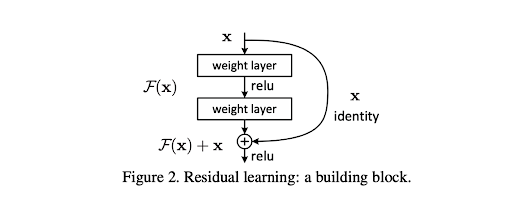
\includegraphics[width=5in]{images/3.1.png} 
   \\\fontsize{11pt}{24pt} Figure 3.1: A residual block.
\end{center}
				

\subsection{MobileNet}
MobileNet is CNN proposed by Howard et al.  \cite{20} that uses depth-wise separable convolutions to design relatively lightweight networks primarily aimed at having smaller sizes while maintaining parity in performance to larger, state-of-the-art models. The primary innovation of MobileNet is a depth-wise separable convolution, which differs from the 2D convolution generally used in other CNNs. 2D convolutions are performed over multiple/all input channels of an image (R,G and B, for example). In depth-wise convolutions, each channel is kept separate and is convolved independently. The output obtained from each channel is stacked together to get the output as a multi-dimensional tensor. Finally then, these output channels are combined to form a set number of channels, adding the separable part to the depth-wise convolution. This process is far more efficient as it requires a far lesser amount of mathematical computation than a regular 2D convolution resulting in faster networks with fewer parameters. 



   








\begin{center}
   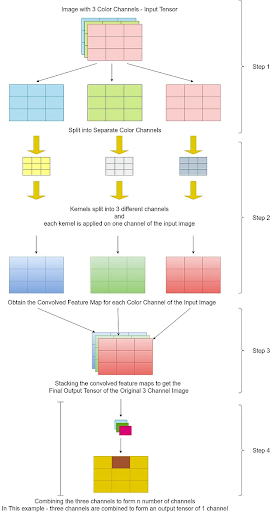
\includegraphics[width=4.5in]{images/3.2.png} 
   \\\fontsize{11pt}{24pt} Figure 3.2: MobileNet convolution.
\end{center}



 


\subsection{DenseNet}
DenseNet (short for a Densely Connected Network), is a CNN proposed by Huang et al.  \cite{21} that uses densely connected layers to pass the feature map of a specific layer to all subsequent layers in the network. The aim of DenseNet was to alleviate the vanishing gradient problem and to strengthen feature propagation via the densely connected layers. DenseNets also require fewer parameters. As each layer receives the output (and representations) of all previous layers, networks can be more compact and can contain fewer channels, allowing for higher size and memory efficiency. DenseNets have been shown to achieve state-of-the-art results on many image-classification problems. 


\begin{center}
   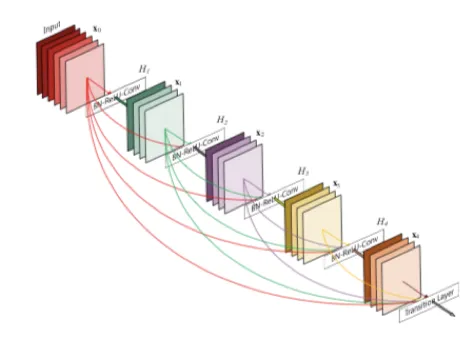
\includegraphics[width=6in]{images/3.3.png} 
   \\\fontsize{11pt}{24pt} Figure 3.3: DenseNet
\end{center}

				
\section{Metaheuristic Algorithms}
Metaheuristic algorithms are techniques for solving optimization problems that are computationally expensive to solve optimally. They aim to generate satisfactorily good solutions that are ideally near-optimal, and are important in problems where the solution space is extremely large and/or requires an inordinate amount of resources in terms of time and computational power to properly solve. These algorithms are stochastic and often contain a degree of randomness in generating new solutions. These algorithms have been of specific research interest because of their ability to avoid early convergence and because of their flexibility in being easily modifiable and applicable to almost any arbitrary optimization problem. These algorithms have been successfully used in various engineering fields such as Power, Infrastructure/Civil Engineering and Communication. 

Metaheuristic algorithms find inspiration from various natural phenomena, and can broadly be classified as following on the basis of their behavior:
Evolutionary Algorithms: Based on genetic evolution in nature, these algorithms involve populations of solutions that are iteratively combined together according to defined procedures to generate newer populations of solutions. The first and most popular algorithm of this sort is the Genetic Algorithm  \cite{9}, based on classical Darwinian evolution. 
Swarm-based Algorithms: These algorithms find their inspiration in the collective large-scale group behavior of natural beings, aiming to mimic their interactions in exploring a solution space for a particular problem. The most popular algorithm of this sort is Particle Swarm Optimization  \cite{10}, based on the behavior of birds. 
Physics-based Algorithms: These algorithms mimic physical phenomena such as gravity to find optimal solutions to a search space. An example is Simulated Annealing  \cite{22}. 
Human-based Algorithms: Similar to swarm-based algorithms, these algorithms are based on the group behaviors of human beings. An example is TLBO  \cite{23}.  

We further discuss some of the algorithms we chose to use for our work.
\subsection{Particle Swarm Optimization}
Particle Swarm Optimization  \cite{10} is a swarm-based metaheuristic algorithm based on the group behavior of birds that was introduced by Kennedy and Eberheart in 1995. This algorithm was theorized on the basis of socio-biological research, which believes that a school of fish/a flock of birds exhibit group movement that benefits from the knowledge of all members in the group. Mimicking this behavior in a solution space can thus lead to close-to-optimal satisfactory solutions for complex optimization problems. 

The algorithm begins with P particles denoting P distinct solutions, with each particle having at any iteration t a position Xi(t) and a velocity Vi(t). Per iteration, the position and velocity of each particle are updated according to the equations (3.1) and (3.2):\\ 
Xi(t + 1) = Xi(t) + Vi(t)          – (3.1)\\ 
Vi(t + 1) = w.Vi(t) + c1.r1.(pbest(i) - Xi(tt)) + c2.r2.(gbest - Xi(t))     - (3.2)\\
where r1 and r2 are random numbers between 0 and 1, c1 and c2 are parameters of the algorithms, \\
pbest(i) is the best position of particle i thus far \\
and gbest is the best solution found thus far. \\
Both subtractions in equation (3.2) are vector subtractions. 


The parameter w is called the inertia weight constant and is between 0 and 1, determining to what extent the new velocity of a particle is dependent upon its previous velocity. The parameters c1 and c2 are respectively called the cognitive and social constants, and denote the weightage given to local and global knowledge in affecting the change in velocity.

\begin{center}
   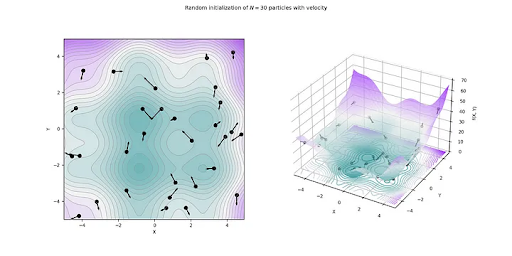
\includegraphics[width=5.5in]{images/3.4.png} 
   \\\fontsize{11pt}{24pt} Figure 3.4: Visualization of PSO
\end{center}



A modified version of PSO called Hierarchical PSO with Time Varying Acceleration Constants (HPSO-TVAC) was introduced by Ghasemi et al.  \cite{24} in  2017.
\subsection{Genetic Algorithm}
The Genetic Algorithm  \cite{9} is an evolutionary metaheuristic algorithm first developed in the 1960s. It mimics darwinian evolution and involves a population of individuals (or solutions), each represented by a certain chromosome consisting of various genes. The fitness (or the objective function that we’d like to optimize) is measured for each individual, and the fittest individuals in the population then ‘reproduce’ to generate new individuals for the next iteration using a process called crossover. To mimic natural evolution, these new individuals can also have random changes via the process of mutation. 


\begin{center}
   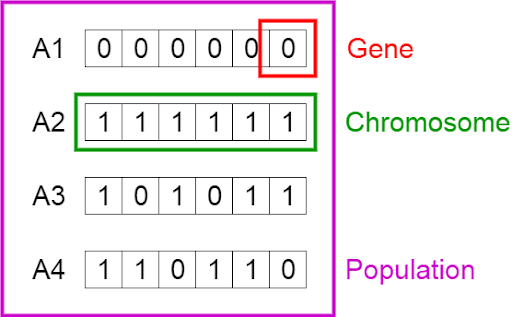
\includegraphics[width=5in]{images/3.5.png} 
   \\\fontsize{11pt}{24pt} Figure 3.5: Genetic Algorithm Representation
\end{center}
			


\begin{center}
   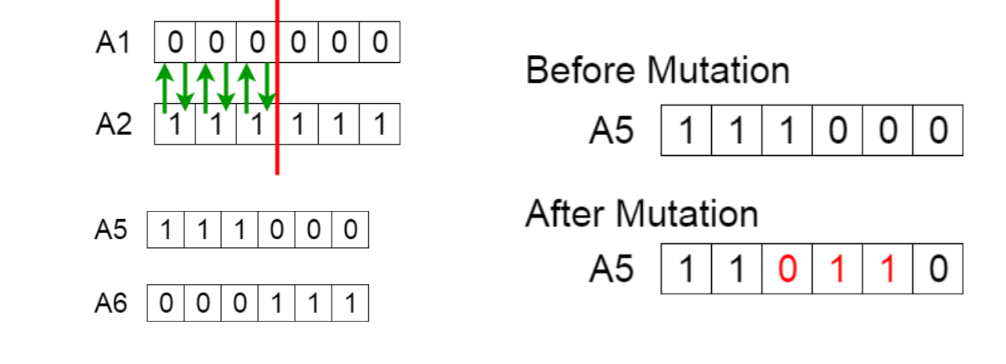
\includegraphics[width=5in]{images/3.6.png} 
   \\\fontsize{11pt}{24pt} Figure 3.6: Crossover and Mutation
\end{center}


We also use several other metaheuristics such as Coral Reef Optimization  \cite{26}. Grey Wolf Optimization  \cite{12} and Harmony Search  \cite{27}.
\section{Feature Selection}
Often, all features of a given dataset are not relevant to the machine learning problem at hand. In these cases, Feature Selection refers to the task of removing the best features from a dataset to increase performance of the model being built. Feature Selection is a critical process in machine learning that is specifically important with data where there exist a significantly large number of features. In such cases, learning often causes overfitting which in turn causes worse generalization and thus worse real-world performance of the model. In these cases, Feature Selection is desirable as it not only increases performance but also decreases computational complexity. Feature selection can be particularly important in the task of image classification. CNNs output feature representations that are significantly large in nature. Often, not all of the features in an image are important to the classification task at hand. For example, in the particular field of AI-generated image detection, AI-generated images have certain marked characteristics that can be more important to the classification task than other more generic features. For instance, AI-generated images often have issues with fingers when generating human portraits, as shown in figure 3.7. In these cases, feature selection can help identify and focus on these aspects of AI-images resulting in better classification accuracy.


\begin{center}
   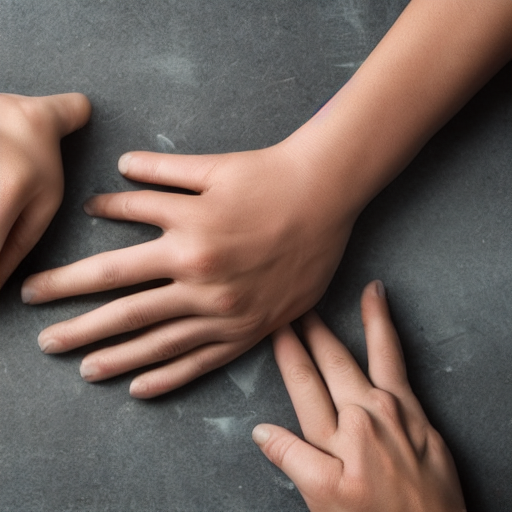
\includegraphics[width=3in]{images/3.7.png} 
   \\\fontsize{11pt}{24pt} Figure 3.7: an AI-generated image of a hand.
\end{center}



Generally, the techniques are classified into three categories: filter, wrapper and embedded methods. Filter methods are independent of the learning algorithm, while Wrapper methods include learning algorithms and train a new model for every feature subset selected. Embedded methods usually consist of some combination of filter and wrapper methods. One of the many wrapper methods is a metaheuristic algorithm, having a long history of being used for this specific application  \cite{13}. 

\chapter{Procedure}

\fontsize{12pt}{24pt}\selectfont  (The code for our work can be found at - https://github.com/artshouldterrify/btpsem8)
We used Kaggle notebooks accelerated by a P100 GPU for all model training. 

\section{Dataset}
CIFAKE: Real and AI-Generated Synthetic Images: This dataset comes from two major research works : - Real images are from Krizhevsky \& Hinton (2009)  \cite{7} , fake images are from Bird \& Lotfi (2024)  \cite{6}.  The dataset contains two classes - REAL and FAKE. For REAL, images were collected from Krizhevsky \& Hinton's CIFAR-10 dataset and for the FAKE images, the equivalent of CIFAR-10 with Stable Diffusion Version 1.4 was generated. There are 100,000 images for training (50,000 per class) and 20,000 for testing (10,000 per class). This is the largest dataset of such AI-generated images to date.

\begin{center}
   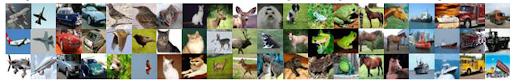
\includegraphics[width=5in,height=1in]{images/4.1.png} 
   \\\fontsize{11pt}{24pt} Figure 4.1: Examples of real images from CIFAR-10 Image Classification Dataset

\end{center}


\begin{center}
   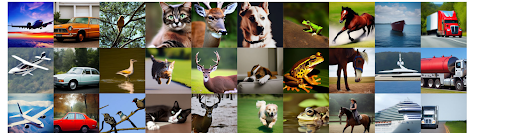
\includegraphics[width=5in]{images/4.2.png} 
   \\\fontsize{11pt}{24pt} Figure 4.2: Examples of AI - Generated images from CIFAKE Dataset
\end{center}



\section{Pre-trained model selection}
In this section, we firstly tested multiple pre-trained models by training and fine-tuning them on 10\% of the dataset. We used a training-testing split of 0.8-0.2 for this portion of the training and we tested models based on ResNet152V2  \cite{19}, NASNetLarge  \cite{25}, DenseNet121  \cite{21} and MobileNetV3Large \cite{28}. We also used a validation set equivalent in size to the testing set, randomly taken from the rest of the dataset. Each of these models uses an input image size of 224x224 and we used 2-neuron dense layer and global 2D-average pooling layer attached to the top of each model with a softmax activation as our classifier. 


We used Keras’ SparseCategoricalCrossentropy as our loss function and the Adam optimizer with an initial learning rate of 0.0001. We also used two callbacks during training, firstly an early stop mechanism stopping training if validation accuracy hasn’t increased for 10 epochs and secondly a learning rate reduction mechanism that reduces the learning if validation accuracy hasn’t improved for 4 epochs. We ran this initial training for 100 epochs per model. After this, we unfroze the top few layers of our base model and fine-tuned the model for another 50 epochs, this time with only the early stopping mechanism and an initial learning rate of 0.00001. 


We input the images directly from the Kaggle notebook’s virtual directory and apply data augmentation using Keras’ preprocessing module. Keras’ ImageDataGenerator utility allows for augmentation to be automatically applied on any data pipeline, allowing for transformations such as rotation, shearing, zoom and vertical/horizontal flips. We used this utility in conjunction with flow\_from\_directory to ultimately create a pipeline that automatically imported data from the virtual directory and simultaneously applied random transformations to it within a set range of parameters that we can define. The parameters we tested for our pipeline are listed in Table 4.1.


    
\begin{table}[H]
\begin{center}
\begin{tabular}{|l|l|l|}
\hline
S.No & Parameter                       & Value \\ \hline
1.   & horizontal flip & True          \\ \hline
2.   & vertical flip      & True          \\ \hline
3.   & rotation range      & 0.5          \\ \hline
4.   & width shift range     & 0.25          \\ \hline
5.   & height shift range     & 0.25          \\ \hline
6.   & shear range     & 0.2          \\ \hline
7.   & zoom range     & 0.4          \\ \hline
\end{tabular}
\end{center}
\caption{Data augmentation parameters}
\end{table}
 
We additionally used the preprocessing\_func parameter of the ImageDataGenerator to apply specific transformations of format that specific pre-trained models required.

\begin{center}
   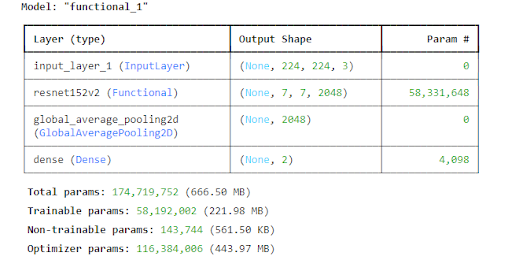
\includegraphics[width=6in,height=3in]{images/4.3.png} 
   \\\fontsize{11pt}{24pt} Figure 4.3: Model Summary
\end{center}

			


We start with the code to define the data input pipeline.
\begin{center}
   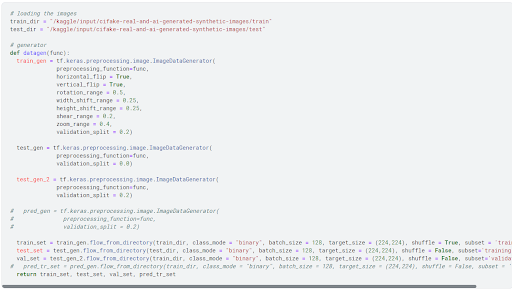
\includegraphics[width=6in,height=5in]{images/c1.png} 
   \\\fontsize{11pt}{24pt} Code: Data pipeline
\end{center}
  
  
We then define the model using Keras’ applications module, which allows us to download pre-trained weights for our base CNNs directly. We define a GlobalAveragePooling2D layer and a 2-neuron softmax Dense layer on top of the model as our classifier.

\begin{center}
   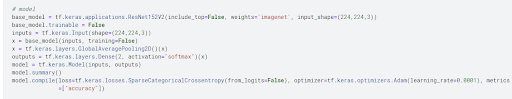
\includegraphics[width=6.5in]{images/c2.png} 
   \\\fontsize{11pt}{24pt} Code: Model definition
\end{center}
  
		
  
We then create instances of the data pipeline, define our callbacks and begin training. 

\begin{center}
   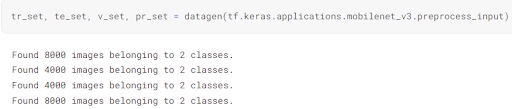
\includegraphics[width=6in]{images/c3.png} 
   \\\fontsize{11pt}{24pt} Code: Pipeline instances
\end{center}

		
\begin{center}
   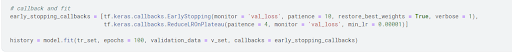
\includegraphics[width=6in,height=1in]{images/c4.png} 
   \\\fontsize{11pt}{24pt} Code: Training
\end{center}
		 

We use the history object created by the .fit function to graph the training process.

\begin{center}
   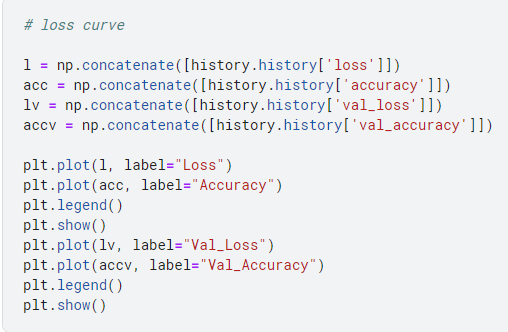
\includegraphics[width=5.5in]{images/c5.png} 
   \\\fontsize{11pt}{24pt} Code: Plotting Training
\end{center}
  
We lastly fine-tuned the model.
\begin{center}
   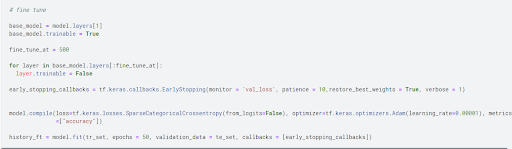
\includegraphics[width=6.5in,height=2in]{images/c6.png} 
   \\\fontsize{11pt}{24pt} Code: Fine Tuning
\end{center}

  
Using this methodology, we trained models based on multiple pre-trained models and accordingly selected the best candidates for our final model. 

\section{Comparison of different metaheuristics}

We picked one of the models trained in section 4.2 and used it to compare different metaheuristic algorithms based on previous comparative studies of metaheuristic algorithms  \cite{13}. For this we used the python library mafese  \cite{28mafese}, a purpose-built library that implements a framework to optimize feature selection problems using multiple methods, including but not limited to metaheuristic algorithms. Mafese is built over another library Mealpy which implements a wide up-to-date range of metaheuristic algorithms. 

To begin, we removed the classifier we had trained over our base CNN (that we picked from the multiple we trained) and processed the same 10\% of the dataset to generate feature representations for training and testing datasets. We then stored these feature representations in a numpy array and define a MhaSelector object, a generalized implementation that allows us to use any metaheuristic we prefer to optimize a generic feature selection problem. This selector trains a separate classifier for any feature subset it explores and outputs the best solution it finds. We iteratively ran this procedure over multiple metaheuristics to find the best algorithm for our data. 

We used a KNN algorithm as our classifier for this step, and we ran each metaheuristic for 50 epochs with a population size of 50. We lastly graphed the results to compare the different algorithms on the number of features selected and the accuracy achieved. 

We start with generating features using our previously defined data pipelines.

\begin{center}
   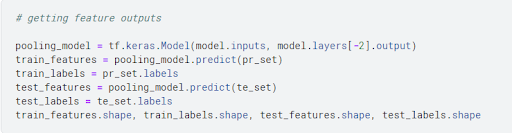
\includegraphics[width=6in,height=2in]{images/c7.png} 
   \\\fontsize{11pt}{24pt} Code: Generating features for metaheuristics
\end{center}

	
 
We then use mafese to iterate over multiple metaheuristics.


\begin{center}
   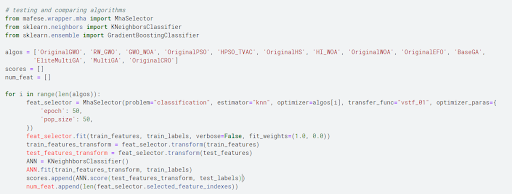
\includegraphics[width=6in,height=3in]{images/c8.png} 
   \\\fontsize{11pt}{24pt} Code: Running metaheuristics
\end{center}

	 
 
We finally plot our results using seaborn.

\begin{center}
   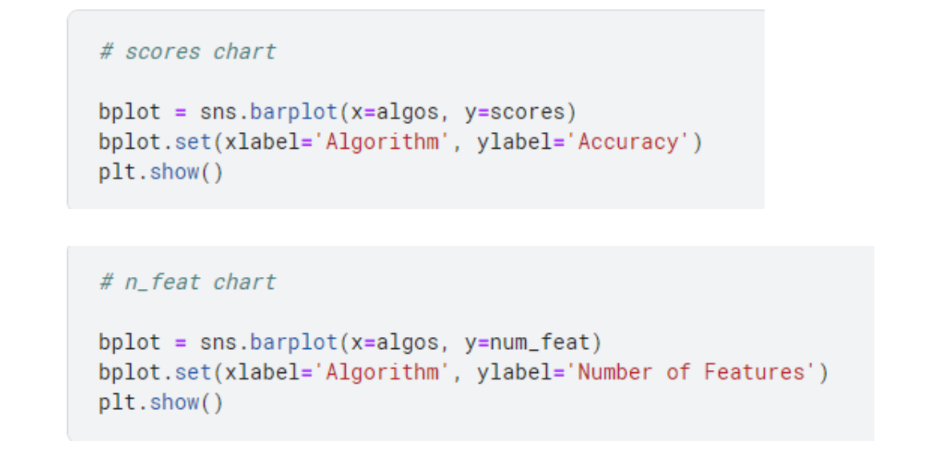
\includegraphics[width=6in]{images/c9.png} 
   \\\fontsize{11pt}{24pt} Code: Comparing number of features and accuracy
\end{center}

	 
		

\section{Final model and applying best metaheuristic}
We then compared the results of the various pre-trained models to select the best model and similarly compared different metaheuristics to select the best fit algorithms. We then trained an entirely new model based on the pre-trained model with the best results, but this time on the entire dataset of 120,000 images. This training was run for 15 epochs and 0.0001 learning rate initially, with the early stopping limit being 3 epochs and the learning rate reduction limit being 2 epochs, post which the model was fine tuned for another 10 epochs with a learning rate of 0.00001. We then applied the best metaheuristic, this time for 20 epochs with a population size of 30. This reduction was due to the larger nature of the training data which induced restrictions on the time we could run the model for. We used the same data pipelines we’d defined initially for this phase of training too. We finally saved the selection of features outputted by our chosen metaheuristic. 

We start with the modified training and testing sets. 

\begin{center}
   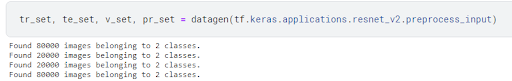
\includegraphics[width=6in]{images/c10.png} 
   \\\fontsize{11pt}{24pt} Code: Training on full dataset
\end{center}

		
  
We then modify training parameters.

\begin{center}
   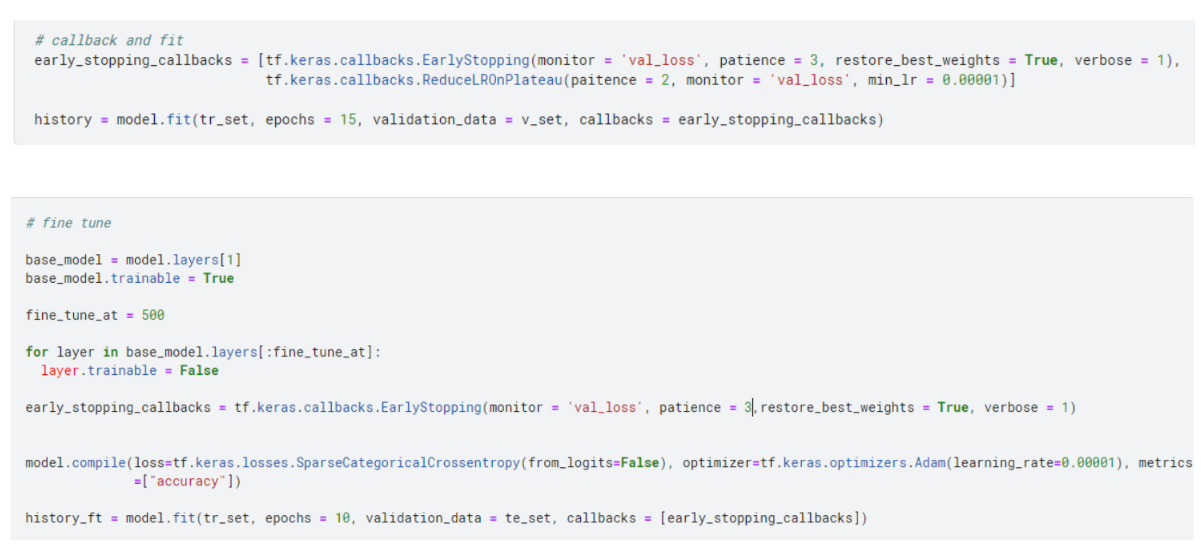
\includegraphics[width=6in,height=3in]{images/c11.png} 
   \\\fontsize{11pt}{24pt} Code: Modified training parameters
\end{center}
		
  
We lastly modify the run the code in figure (xix) to generate training and testing features and apply our metaheuristics with two modifications. Firstly, instead of using the KNN algorithm, we use a Multi-Layer Perceptron as our final classifier and secondly, we run the algorithms for only 20 epochs with a population size of 30.

\begin{center}
   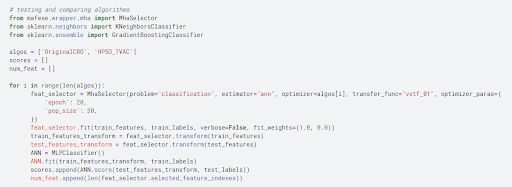
\includegraphics[width=6in, height=3in]{images/c12.png} 
   \\\fontsize{11pt}{24pt} Code: Final metaheuristic
\end{center}
		
		
  
We finally save the feature subset selected by our algorithm.


\begin{center}
   \includegraphics[width=5in]{images/c13.png} 
   \\\fontsize{11pt}{24pt} Code: Saving selected features
\end{center}
		
		

\chapter{Results and Discussions}
\section{Preliminary model results}

\fontsize{12pt}{24pt}\selectfont We tried models based on 5 different pre-trained models - ResNet50V2, ResNet152V2, NASNetLarge, MobileNetV3Large and DenseNet121. Of these, we found the best performing to be ResNet152V2 with a training accuracy of 97.65\% and a testing accuracy of 94.42\%. We additionally measured the models on their recall, precision and F1-score. \\
Accuracy = TP + TN/TP +TN + FP + FN					-  (5.1)\\
Specificity = TN/TN + FP							-  (5.2)\\
Precision = TP/TP + FP						    	-  (5.3)\\
F1-Score = 2(Precision x Recall)/(Precision + Recall) -  (5.4)\\
where TP denotes a True Positive, TN denotes a True Negative, FP a False Positive and FN a False Negative. For this task the positive class (1) is a real image and the negative class (0) is an AI-generated image.
\begin{table}[H]
\begin{center}
\begin{tabular}{|l|l|l|l|l|}
\hline
Model & Accuracy  & Precision & Specificity & F1-Score\\ \hline
ResNet50V2   & 0.9047 & 0.9016 & 0.9032 & 0.9008         \\ \hline
ResNet152V2   & 0.9417 & 0.94285 & 0.943 & 0.9416      \\ \hline
NASNetLarge  & 0.89425 & 0.9104 & 0.9140 & 0.89211      \\ \hline
DenseNet121   & 0.90675 & 0.90332 & 0.9025 & 0.90714      \\ \hline
MobileNetV3Large   & 0.9032 & 0.91983 & 0.9230 & 0.9013      \\ \hline

\end{tabular}
\end{center}
\caption{Initial Training Results}
\end{table}

\begin{center}
   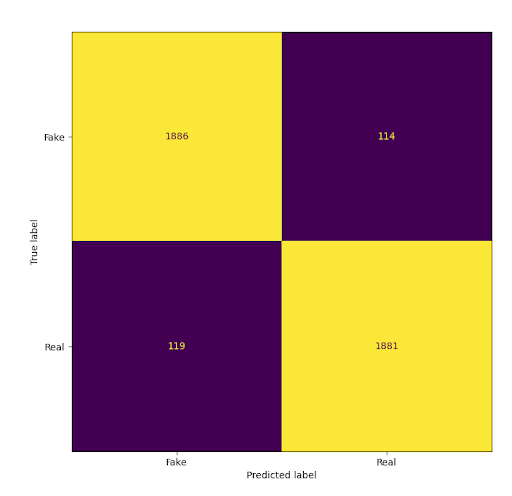
\includegraphics[width=6in, height=5in]{images/5.1.png} 
   \\\fontsize{11pt}{24pt} Figure 5.1: Confusion Matrix of best model: ResNet152V
\end{center}

	
\begin{center}
   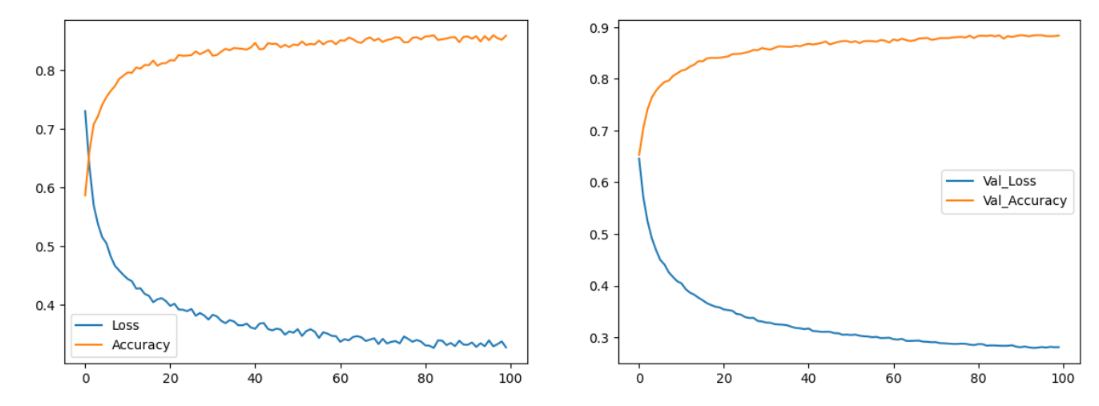
\includegraphics[width=6in, height=2.5in]{images/5.2.png} 
   \\\fontsize{11pt}{24pt} Figure 5.2: Training ResNet152V2 with top layers frozen
\end{center}

\begin{center}
   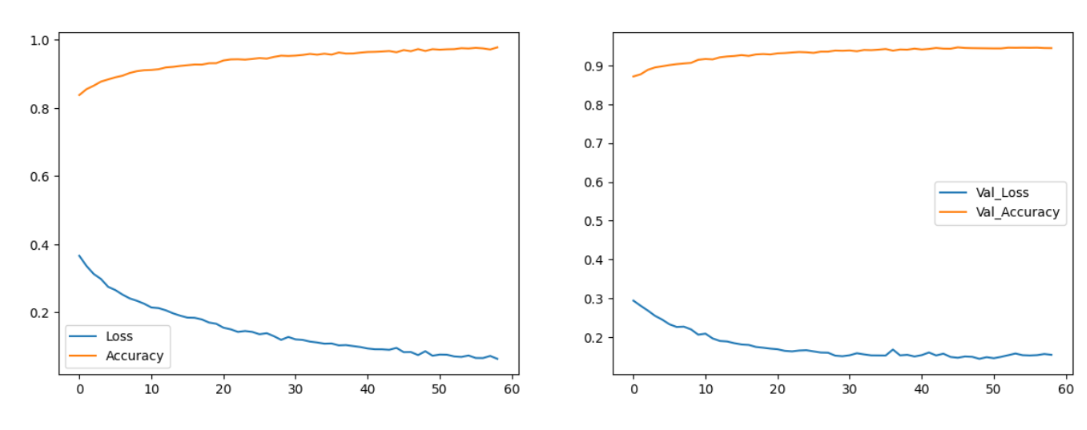
\includegraphics[width=6in, height=2.5in]{images/5.3.png} 
   \\\fontsize{11pt}{24pt}	Figure 5.3: Fine-tuning ResNet152V2 with top layers unfrozen
\end{center}


	

\section{Preliminary metaheuristic comparison}
We tried 13 metaheuristic algorithms initially- Grey Wolf Optimization and RWGWO  \cite{12} \cite{29}, Grey Wolf/Whale Optimization Hybrid  \cite{30}, PSO  \cite{10}, HPSO-TVAC  \cite{24}, Harmony Search  \cite{27}, Whale Optimization and HI-WOA  \cite{31} \cite{32}, Electromagnetic Field Optimization  \cite{33}, Genetic Algorithm and 2 other advanced variants of the GA  \cite{9} and Coral Reef Optimization  \cite{26}. We trained these algorithms using features from the MobileNetV3Large model we had previously trained. We measured only a single metric, accuracy (equation 5.1) for these algorithms. The results are presented in tabular and graphical form.

\begin{center}
   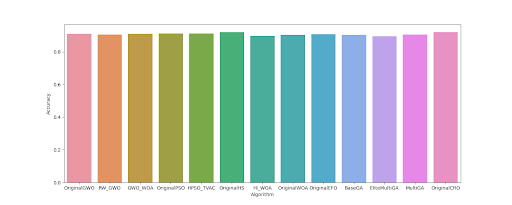
\includegraphics[width=7in, height=2.5in]{images/5.4.png} 
   \\\fontsize{11pt}{24pt}	Figure 5.4: Graphic results of metaheuristic comparison
\end{center}
\begin{table}[H]
\begin{center}
\begin{tabular}{|p{1cm}|p{4cm}|p{2cm}|}
\hline
S.No & Algorithm           & Accuracy\\ \hline
1.   & Grey Wolf Optimization & 0.9105          \\ \hline
2.   & RW-GWO      & 0.906          \\ \hline
3.   & Grey Wolf/Whale Optimization      & 0.90975          \\ \hline
4.   & PSO     & 0.913         \\ \hline
5.   & HPSO-TVAC     & 0.9125          \\ \hline
6.   & Harmony Search     & 0.9205          \\ \hline
7.   & HI-WOA     & 0.8975          \\ \hline
8.   & Whale Optimization     & 0.90375          \\ \hline
9.   & Electromagnetic Field Optimization     & 0.908          \\ \hline
10.   & Genetic Algorithm     & 0.90375          \\ \hline
11.   & Multi-Objective Elite GA     & 0.899575          \\ \hline
12.   & Multi-Objective GA     & 0.906          \\ \hline
13.   & Coral Reef Optimization     & 0.9205          \\ \hline
\end{tabular}
\end{center}
\caption{Metaheuristic Comparison}
\end{table}

We therefore use Coral Reef Optimization as our primary metaheuristic algorithm.

\section{Final Model and Metaheuristic feature selection}
We finally trained a ResNet152V2 model and used Coral Reef Optimization for feature selection, achieving an initial testing accuracy of 96.933\% after fine-tuning the model and a testing accuracy of 97.315\%. The associated training graphs and results are shown below. We calculate all relevant and previously mentioned metrics alongside a confusion matrix and an ROC curve.


\begin{center}
   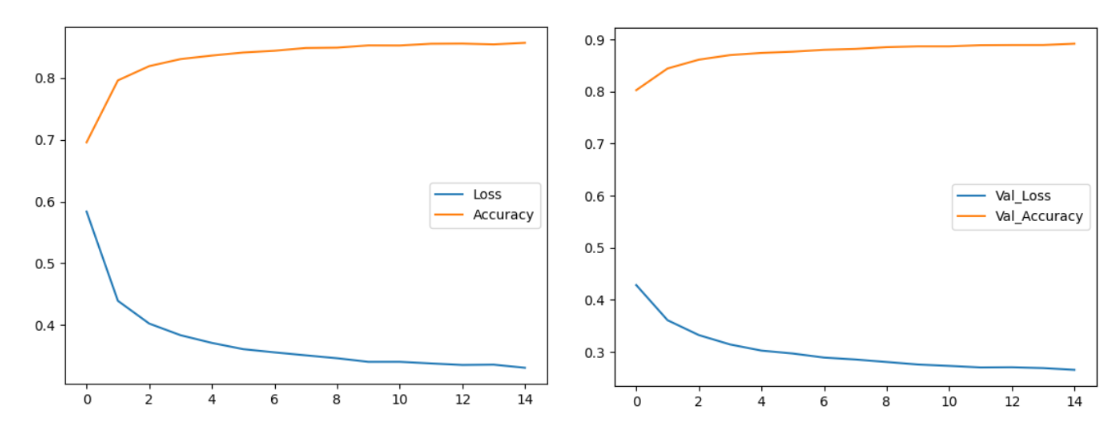
\includegraphics[width=6in, height=2.5in]{images/5.5.png} 
   \\\fontsize{11pt}{24pt}	Figure 5.5: Training the final model with top layers frozen
\end{center}


\begin{center}
   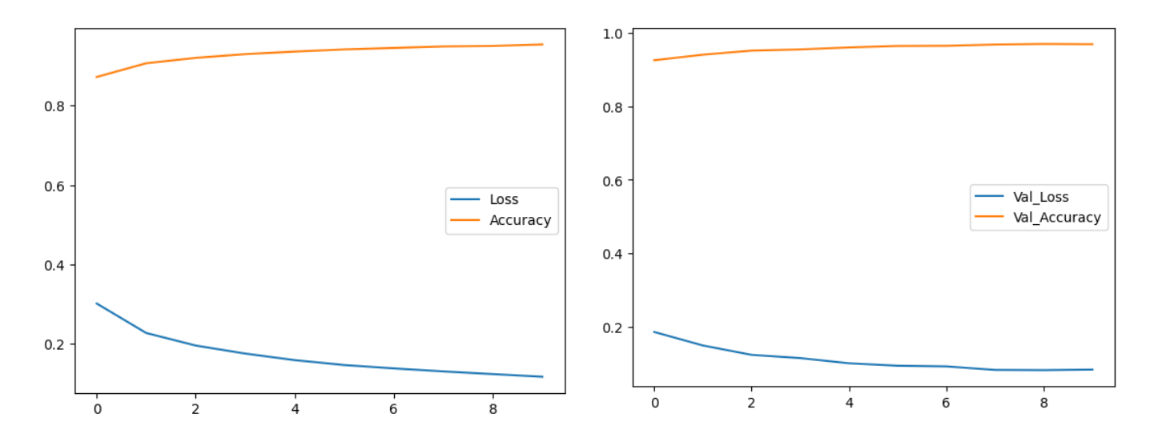
\includegraphics[width=6in, height=2.5in]{images/5.6.png} 
   \\\fontsize{11pt}{24pt}	Figure 5.6: Fine-tuning the final model with top layers unfrozen
\end{center}
			
\begin{center}
   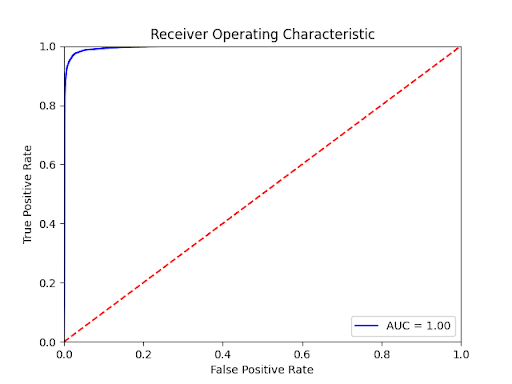
\includegraphics[width=5.5in]{images/5.7.png} 
   \\\fontsize{11pt}{24pt}	Figure 5.7: Receiver Operating Characteristic
\end{center}

\begin{center}
   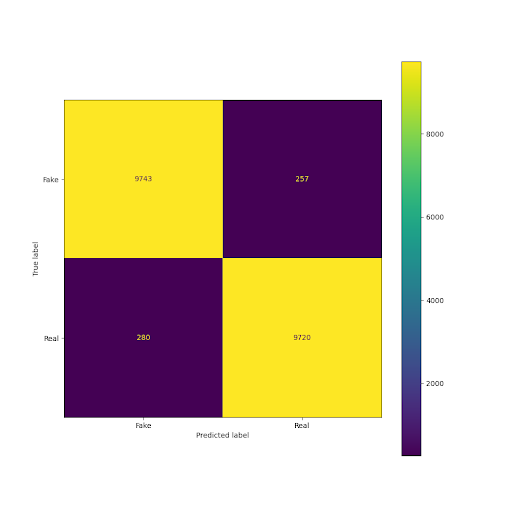
\includegraphics[width=5in,height=4in]{images/5.8.png} 
   \\\fontsize{11pt}{24pt}	Figure 5.8: Confusion Matrix for the Final Model
\end{center}
			

\begin{table}[H]
\begin{center}
\begin{tabular}{|l|l|l|}
\hline
S.No & Parameter                       & Value \\ \hline
1.   & Accuracy & 0.97315          \\ \hline
2.   & Specificity      & 0.9743          \\ \hline
3.   & Precision      & 0.97424          \\ \hline
4.   & F1-Score     & 0.97311          \\ \hline
5.   & ROC-AUC Score     & 0.99571          \\ \hline

\end{tabular}
\end{center}
\caption{Final Results}
\end{table}


		





\chapter{Findings and Conclusion}


\begin{itemize}
    \item Relevant literature was thoroughly examined and the connections between past research and our problem statement were identified. This enabled us to devise a methodology for expanding upon previous work to achieve our objectives.
    \item We found and used an extensive dataset CIFAKE containing contrasting Real images and fake AI-generated synthetic images. This dataset contains 120,000 images in total with 60,000 images belonging to each class, i.e., Real and Fake.

    \item We used state-of-the-art transfer learning models - ResNet50\_V2, ResNet152\_V2, NASNetLarge, DenseNet121 and MobileNetV3Large with ResNet152\_V2 giving the best results, a testing accuracy of 94.42\%.

    \item We also improved performance metrics using Coral Reef Metaheuristic optimization algorithm for feature selection and achieved accuracy of 97.315\%.

    \item All the theoretical aspects and procedures discussed in Chapter 3 and Chapter 4 respectively were successfully demonstrated and their performance results were noted in Chapter 5 hence proving the feasibility and applicability of the proposed work.
\end{itemize}


\newpage
\addcontentsline{toc}{chapter}{REFERENCES}




\begingroup
\renewcommand\bibname{References}

\renewcommand{\section}[2]{}%
\bibliographystyle{ieeetr} % Change to the desired style
\bibliography{references} % Specify your .bib file name without the extension

\endgroup

\newpage


\addcontentsline{toc}{chapter}{PLAGIARISM}

\thispagestyle{plain}
\begin{center}
\large \large {PLAGIARISM REPORT}

\end{center}

\begin{center}
   \includegraphics[width=7in]{images/p1.JPG} 
\end{center}


\begin{center}
   \includegraphics[width=7in]{images/p2.JPG} 
\end{center}


\begin{center}
   \includegraphics[width=7in]{images/p3.JPG} 
\end{center}


\begin{center}
   \includegraphics[width=7in]{images/p4.JPG} 
\end{center}


\begin{center}
   \includegraphics[width=7in]{images/p5.JPG} 
\end{center}

\newpage

\addcontentsline{toc}{chapter}{APPENDIX}
\thispagestyle{plain}
\begin{center}
\large \large {APPENDIX}

\end{center}

[1] Computation Library - Numpy: https://numpy.org/

[2] Computation Library - SciPy: https://scipy.org/ 

[3] Machine Learning Library - SKLearn: https://scikit-learn.org/stable/ 

[4] Machine Learning Library - Tensorflow: https://www.tensorflow.org/

[5] Machine Learning Library - Keras: https://keras.io/

[6] Metaheuristic Framework Library - MealPy: https://pypi.org/project/mealpy/

[7] Metaheuristic Framework Library - Mafese: https://pypi.org/project/mafese/0.1.4/

[8] Plotting Library - MatPlotLib: https://matplotlib.org/

[9] Plotting Library - Seaborn: https://seaborn.pydata.org/

[10] Dataset hosting and model training - Kaggle: https://www.kaggle.com/

% Similarly create more chapters here


% \newpage
% The bibliography goes under a separate .bib file. To quote articles, just fill the appropriate headings in the bibliography file. 

\end{document}
